\documentclass[14pt]{beamer}
\usetheme{Antibes}
\definecolor{myOrange}{RGB}{238,97,53}
\setbeamercolor*{palette primary}{fg=myOrange}
\setbeamercolor*{palette secondary}{fg=myOrange,bg=white}
\setbeamercolor*{palette tertiary}{bg=myOrange,fg=white}
\setbeamercolor*{titlelike}{parent=palette primary}
\setbeamercolor*{itemize item}{fg=myOrange}
\setbeamercolor{block title example}{bg=myOrange} 
\setbeamercolor{section in toc}{fg=black}
\setbeamertemplate{sections/subsections in toc}[sections numbered]
\setbeamercolor{section number projected}{bg=myOrange,fg=yellow}
\setbeamertemplate{footline}[frame number]
\setbeamertemplate{frametitle}{
  \begin{centering}
  \insertframetitle
    \par
    \end{centering}
}
\setbeamertemplate{itemize item}{\textbullet}

\usepackage{amsmath}
\usepackage{ulem}
\usepackage{alltt}
\usepackage[english]{babel}
\usepackage{listings}
\usepackage{hyperref}
\logo{
\includegraphics[width=1cm]{logo.png}}
\newcommand\B{\rule[-1.7ex]{0pt}{0pt}}
\def\colored#1{\textcolor{myOrange}{#1}}

\setcounter{tocdepth}{1}

\begin{document}
\title{Cucumber-flavored Java}
\author{Arkady Galyash}
\institute{dxChartPro}
\date{\today}

\newcommand{\smaller}[1] {
  {\scriptsize {#1}}
}

% Здравствуйте, меня зовут Аркадий Галяш, я работаю в команде dxChartPro. 
% Сегодня я представляю вашему вниманию презентацию на тему "Java со ввкусом огурца", посвященную проблемам и преимуществам использования инструментария BDD в реальных проектах
% Вопросы можно задавать как походу доклада, так и в конце.
% Сначала хотелось бы уточнить, что бдд в последнее время очень популярная тема и многие доклады ей посвященные этому вопросу имеют некоторый маркетинговый оттенок, но этот я постарался сконцентрироваться на технической стороне вопроса
% Так что доклад вышел даже не столько про бдд, сколько про то, как можно применять его инструментарий. =)
% Вопросы к аудитории:
% Кто работает по TDD?
% Кто слышал о TDD?
% Кто использует BDD?
% Кто слышал\писал сценарии для BDD?
\frame{\titlepage}

% Сегодня мы рассмотрим следующие вопросы:
% 1) Что такое BDD? О чем вообще пойдет речь? Кратко, но содержательно
% 2) Зачем оно нам понадобилось в dxChartPro? И что хорошего оно принесло в разработку?
% 3) Какие трудности и подводные камни поджидают тех, кто собирается его использовать? С чем мы столкнулись?
\frame%
{\frametitle{Agenda}
  \tableofcontents[1]
}

% Ок, а что такое бдд? Его придумал ден нортн в 2006 году.
% в то время, когда проводил тренинги по тдд
% он же реализовал JBehave - первый фреймворк для бдд
% Наибольшее признание техника бдд получила у руби-коммьюнити, поэтому и наиболее известный фреймворк для бдд - из руби(огурец)
\section{What is BDD?}
\subsection{BDD history}
\frame{\frametitle{BDD history}
  \begin{itemize}
    \item Behavior-driven development
    \item Dan North, 2006
    \item Invented BDD while teaching TDD
    \item JBehave - first BDD framework
    \item Ruby: RSpec, Cucumber
  \end{itemize}
}

% Как выглядит бдд - как тдд, только добавляется еще один шаг:
% перед написанием юнит-тестов, пишутся еще и спецификации в текстовом формате с небольшими ограничениями
% Эти спецификации состоят из юзер сторий
% Которые вначале описывают: кто, что-то делает, зачем и что из этого он хочет получить
% и наиболее важная часть юзер стории - набор сценариев
\subsection{What BDD looks like?}
\frame{\frametitle{What BDD looks like?}
  \begin{itemize}
    \item Specification consists of user stories
    \item Narrative
      \begin{itemize}
        \item Who is a stackholder?
	\item Which effect the stakeholder wants to have?
	\item What value will be derived from this effect?
      \end{itemize}
    \item User story is a collection of scenarios
    \item Scenario is a sequence of sentences which start with BDD Keywords
  \end{itemize}
}

% Сценарии - последовательность пред и пост условий и событий.
\subsection{BDD Keywords}
\frame{\frametitle{BDD Keywords}
  \begin{itemize}
    \item Preconditions - \colored{Given} ...
    \item Events - \colored{When} ...
    \item Postconditions - \colored{Then} ...
  \end{itemize}
}

% Давайте рассмотрим в качестве примера - Винни-Пуха, тестирующего пчел на правильность.
\subsection{Winnie Example}
\frame{\frametitle{Winnie Story}
  \begin{columns}
    \column{.5\textwidth}
      \begin{flushleft}
      {\fontfamily{ttfamily}\selectfont
	  \colored{Story}: Steal honey from bees \\
	  \colored{ }\\
	  \colored{Narrative:} \\
	  \colored{In order to} get honey \\
	  \colored{As a} Winnie-the-Pooh  \\
	  \colored{I want to} steal honey 
      }
      \end{flushleft}
    \column{.5\textwidth}
      
\includegraphics[width=\textwidth]{winnie.png}
  \end{columns}
}

\frame{\frametitle{Winnie Scenario}
  \begin{columns}
    \column{.5\textwidth}
      \begin{flushleft}
      {\fontfamily{ttfamily}\selectfont
	\colored{Given} a blue baloon \\
	\colored{When} I fly to bees \\
	\colored{And} I'm singing cloudlet song \\
	\colored{Then} bees will thought that I'm a cloud \\
	\colored{And} I can steal honey 
      }
      \end{flushleft}
    \column{.5\textwidth}
      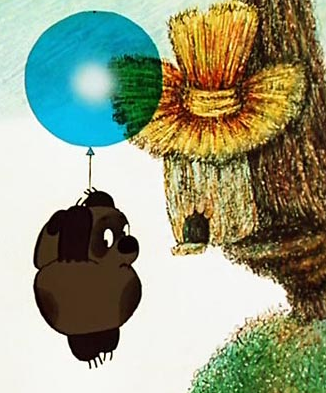
\includegraphics[width=0.85\textwidth]{winnie_and_bees.png}
  \end{columns}
}

% А теперь самое интересное для программистов, при помощи простейших действий обычно это бдд спецификации превращаются в интеграционные тесты.
% О том что именно это за "простейшие действия" мы более детально рассмотрим в тертьей части данной презентации
\subsection{Integration tests}
\frame{\frametitle{Integration tests}
  \begin{itemize}
    \item With little ``BDD magic'' requirements in such format can be used as integration tests
    \item Details in 3rd part (How to use BDD in Java?)
  \end{itemize}
}

% Соответсвенно, мы выяснили, что есть такое бдд, теперь вторая часть - зачем оно нужно.
% Итак, зачем оно нам понадобилось в проекте dxchartpro?
% Ответ прост - до этого мы работали в проекте тосчарт.
\section{Why BDD?}
%\subsection{Why dxChartPro uses BDD-tools?}
%\frame{\frametitle{Why dxChartPro uses BDD-tools?}
%  \begin{center}
%  \only<2>{\huge We worked in TosChart}
%  \end{center}
%}

% Что это значит?
% Например, в тхинкскрипте(внутри тосчарта) можно найти джиюнит тесты, которые не являются по сути юнит-тестами
% И результат, которых не очивиден. То есть у нас было не раз - радает такой тест и ты мучаешься-думаешь почему изменился 6 знак после запятой, а потом автор теста говорит, что текущее поведение правильное, а предыдущее - не верное
% Вообщем, намучавшись с такими тестами, мы поняли, что такие тесты нам не нужны.
%\frame{\frametitle{HowNotTo write Unit-tests}
%  \begin{center}
%    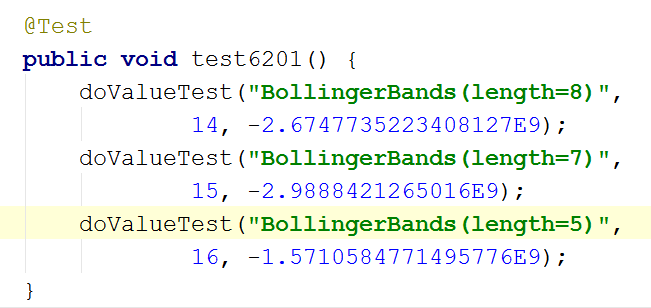
\includegraphics[width=0.9\textwidth]{bad_tdd.png}
%  \end{center}
%}

% Кроме того, чарты - довольно специфический проект с очень слабо специфицированными требованиями.
% Часто на вопрос - как это должно выглядеть - "оно должно вышлядеть красиво"
% Но мы пишем чарты, и довольно много. Кто-нибудь знает сколько чартов написано в девекспертс?
\frame{\frametitle{Chart specifics}
  \begin{itemize}
    \item Charts are not easy to write requirements for
    \item Sometimes it is just ``It should be pretty''
  \end{itemize}
}

% Я лично не знаю, но знаю, что точно более 5.
% Есть тосчарт, на джаве для тоса.
% Есть пачка мобильных чартов
% Есть флексовый дхчартс
% Есть хтмл5 чарты
% И есть наконец наши тоже джавовские чарты
\subsection{Charts in Devexperts}
\frame{\frametitle{How many charts in Devexperts?}
  \begin{itemize}
    \item TOS Charts
    \item Charts in dxMobile
    \item dxCharts
    \item dxChart5
    \item dxChartPro
    \item ...
  \end{itemize}
}

% То есть у нас есть 5 имплементации и они делают плюс-минус одно и тоже: показывают бары, рисуют дравинги, считают стадисы.
% Понятно, что вряд ли мы можем джава код переиспользовать во флексовых чартах
% Но и требования-то примерно одинаковые!
% Более того, если я ничего не путаю, то флексовые чарты писались с оглядкой на тосчарт
% ХТМЛ5 чарты - с оглядкой на флекс
% И так далее, то есть требования были "сделайте нам точно такое же только не на флексе, а на ХТМЛ5", к примеру
\frame{\frametitle{How many charts in Devexperts?}
  \begin{itemize}
    \item dxCharts like TOS Charts, but on Flex
    \item dxChart5 like dxCharts, but on HTML5
    \item dxChartPro like dxCharts, but on Java
    \item Charts in dxMobile like dxChartPro, but on mobile devices
  \end{itemize}
}

% Возьмем к примеру метки на временной оси.
% У всех чартов есть временная ось, на которой располагаются сетки различных дат
% Разумно предположить, что 5 чартов внутри одной компании должны пользоваться одним и тем же аглоритмом расположения меток.
% Ну на крайний случай, требования точно одинаковые, значит и поведение должно быть одинаковое
% На самом же деле все 5 имеют различия, где-то больше, где-то меньше
% Причем понятно, что тут как раз нет вины разработчиков. 
% Просто это только в сказках можно "пойти туда, не знаю куда, принести то, не знаю что". 
\frame{\frametitle{Time axis marks}
  \begin{itemize}
    \item Base feature of trading charts
    \item Main requirement: ``It should look nice''
    \item \only<1>{Are all implementations looks alike?}
      \only<2>{No, different versions have different bugs}
  \end{itemize}
}

% Что же делать? Поэтому нужны требования: а особенно в такой ситуации, когда требования трудно описать формально, лучше и легче всего начать с описания сценариев
\subsection{Write stories}
\frame{\frametitle{How to solve this problem?}
  \begin{center}
    \only<2>{\huge Write a story about it!}
  \end{center}
}

% Плюсов тут огромное количество: например, мы получим хоть какой-то общий знаменатель для всех наших чартовых имплементации
% Плюс все эти спецификации можно будет использовать как тесты для всех проектов
% А т.к. сценарии - это просто текст на английском языке, и для их написания гораздо более важно понимание предметной области, чем умение программировать, а это значит, что читать и писать их могут и юзабилисты и аналитики и куа
% Для программистов - это вообще просто мечта, наконец-то понятно, что нужно писать, плюс еще и тестов тебе уже написали
\frame{\frametitle{Pros}
  \begin{itemize}
    \item We can share requirements between charts implementations (if we want to)
    \item It's plain text, it can work as integration tests with Java, Ruby, JavaScript, C++, Flex, etc.
    \item Not only developer can write/read it:
      \begin{itemize}
        \item analyst/customer wants a feature
        \item QA finds a bug 
      \end{itemize}
  \end{itemize}
}

% Теперь, когда, я надеюсь, я вас убедил, что бдд и вам тоже срочно необходимо, давайте рассмотрим как его организовать в джава, например
% Сначала надо выбрать бдд фреймворк, при помощи которого мы будем преобразовывать спецификации в интеграционные тесты
% Для джавы их существует огромное количество
% Но если отбросить все, которые записывают спецификации в формате отличном от простого текста,
% а также все, без поддержки в иде(полгода назад)
% то останется только джибехейв
\section{How to use BDD in Java?}
\subsection{Choose tool}
\frame{\frametitle{Choose tool}
  \begin{itemize}
    \item \only<1>{Concordion} \onslide<2->{\sout{Concordion (HTML)}}
    \item \only<1-2>{Cucumber-jvm} \onslide<3->{\sout{Cucumber-jvm}}
    \item \only<1>{Instinct} \onslide<2->{\sout{Instinct (Java)}}
    \item JBehave
    \item \only<1>{Spock} \onslide<2->{\sout{Spock (Groovy)}}
    \item ...
  \end{itemize}
}

% Итак, как же превратить спецификации в интеграционные тесты при помощи джибехейв?
% конечно же при помощи аннотаций для методов.
% Основные, Given, When и Then соответсвуют пост, пред условиям и дейтсвиям
% В качестве значения у этих аннотаций нужно указать строку, описывающую, чему именно этот метод соответсвует.
% Внутри этой строки можно пометить места, для связи параметров метода с изменяемой частью строки
% Кроме того, необходимо создать конфигуратор для запуска историй
\subsection{JBehave}
\frame{\frametitle{JBehave}
  \begin{itemize}
    \item POJO with step definitions
    \item Scenario steps map to Java methods via annotations (@Given, @When, @Then, etc.)
    \item $\$parameterName$, $<parameterName>$
    \item Configure story runner
  \end{itemize}
}

% Давайте рассмотрим на примере
% Предположим, мы написали вот такую историю
% Чтобы она заработала, нам необходимо завести соответсвующие методы с нужными аннотациями
\frame{\frametitle{JBehave Story}
  \begin{center}
    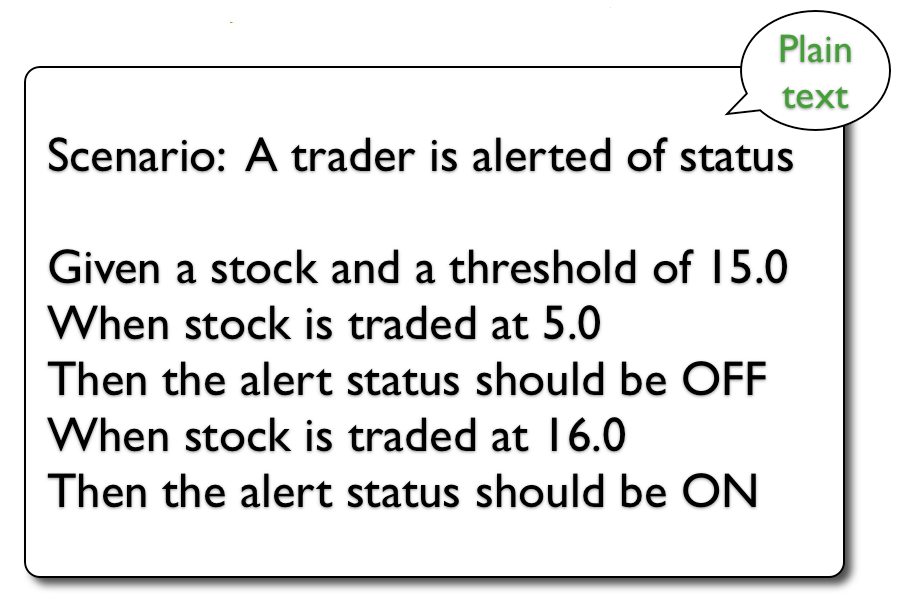
\includegraphics[width=0.9\textwidth]{1.png}
  \end{center}
}

% Т.к. мы захотим вариировать значения для алерта, имеет смысл замести параметр трешхолд
% Количество параметров в строке должно соответсвовать количесву параметров метода: как вы видите, так можно связывать и строковые и примитивные типа. 
\frame{\frametitle{JBehave StepDef}
  \begin{center}
    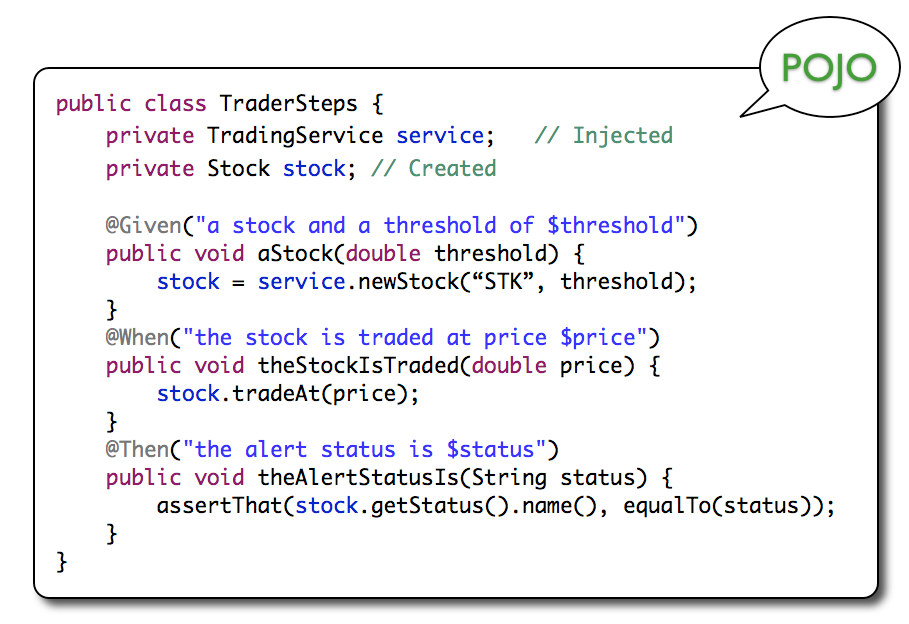
\includegraphics[width=0.9\textwidth]{2.png}
  \end{center}
}

% Кроме уже упомянутых given when then аннотаций, могут быть полезные алиас(ы) если вы хотите связать один метод с несколькими шагами
% А также классические бефоре и афте, которые будут вызываться дл и после соотвественно сценария и истории
\subsection{JBehave Annotations}
\frame{\frametitle{JBehave Annotations}
  \begin{itemize}
    \item @Given
    \item @When
    \item @Then
    \item @Alias, @Aliases
    \item @BeforeScenario, @AfterScenario
    \item @BeforeStory, @AfterStory
  \end{itemize}
}

% Кроме этого, если вам нужно записать более структурированные параметры шага - можно использовать табличные параметры, первая строка - имена столбцов, остальное значения записей.
% Соответсвенно для этого параметром метода должно быть ExamplesTable,чтобы таблица распарсилась
\subsection{Tabular Parameters}
\begin{frame}[fragile]
\frametitle{Tabular Parameters}
\begin{itemize}
\item \begin{lstlisting}[morekeywords={Given,When,Then}, basicstyle=\small\ttfamily, keywordstyle=\color{myOrange}]
Given the users:
| login | password |
| Larry |    123   |
|  Moe  |  qwerty  |
| Curly | password |
When we delete user with login "Curly"
Then the users are:
| login | password |
| Larry |    123   |
|  Moe  |  qwerty  |
\end{lstlisting}
\item ExamplesTable
\end{itemize}
\end{frame}

% Конфигурация для джбехейва выглядит пострашнее, но прелесть в том, что ее можно написать один раз и забыть, мы свою уже полгода не изменяли 
\subsection{JBehave}
\frame{\frametitle{JBehave Configuration}
  \begin{center}
    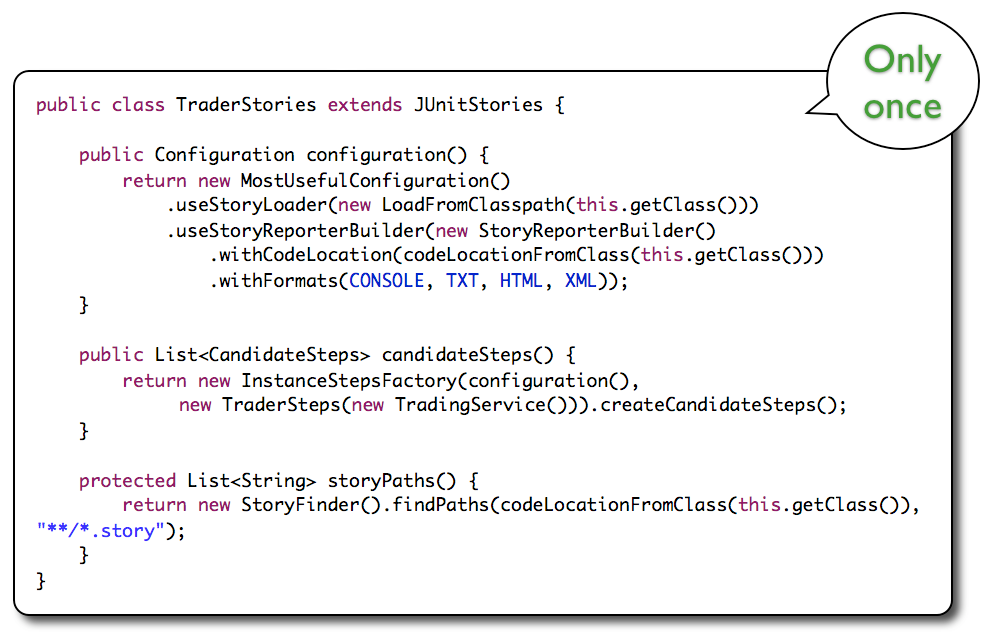
\includegraphics[width=0.9\textwidth]{3.png}
  \end{center}
}


% джибехейв умеет генерировать результаты в различных форматах, например в хтмл
% И имеет еще огромное количество различных функции, облегчающих работу с ним, например, параметризованные сценарии, но это уже слишком джибехейв специфичные вещи
\frame{\frametitle{JBehave Output}
  \begin{center}
    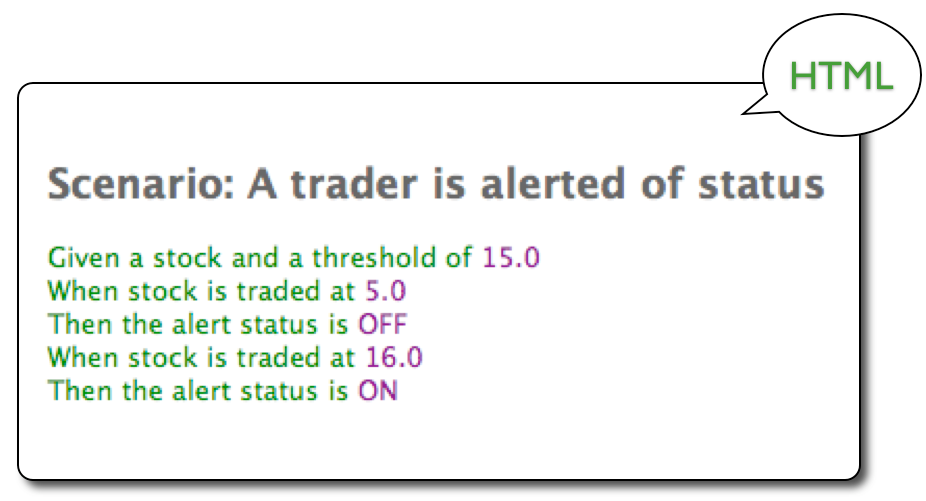
\includegraphics[width=0.9\textwidth]{5.png}
  \end{center}
}

% Что подводит нас к вопросу инфраструктуры - если вы решились использовать джибехейв в своем проекте, что может облегчить вам жизнь при работе с ним?
% Конечно, он поделен на артефакты и легко может быть использован при помощи мавена
% Т.к. проект уже достаточно зрелый, есть интеграции с идеей
% Есть интеграция с хадсоном и что их можно подружить с тимсити, что более актуально для нашей компании
% Кроме того, есть такой забавный проект, который мимикрирует джибехейв тесты под джиюнит, что позваляет запускать их в любой иде так же внешне как джиюнит
\subsection{JBehave infrastructure}
\frame{\frametitle{JBehave infrastructure}
  \begin{itemize}
    \item Maven
    \item IntelliJ support
    \item TeamCity
    \item JBehave JUnit Runner
  \end{itemize}
}

% Подробнее про идеювскую интеграцию: есть поддержка синтаксиса, навигация к методу, соответсвующему шагу и автодополнение
\subsection{IntelliJ support}
\frame{\frametitle{IntelliJ support}
  \begin{center}
      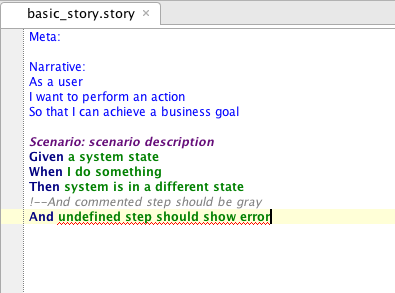
\includegraphics[width=0.8\textwidth]{idea.png}
  \end{center}
}

% Как сделать подружить джибехейв с тимсити?
\subsection{TeamCity support}
\frame{\frametitle{TeamCity support}
  \begin{itemize}
    \item Run your stories as a part of CI
    \item Create TeamCity artifact
    \item Create TeamCity custom tab
  \end{itemize}
}

\subsection{What to test?}
\frame{\frametitle{What to test?}
  \begin{itemize}
    \item dxChartPro - Swing component
    \item JBehave stories - integration tests
    \item Lets test all parts of MVC
  \end{itemize}
}

\subsection{What is the problem?}
\frame{\frametitle{What is the problem?}
  \begin{itemize}
    \item Different Locale (ru\_RU - on my PC, en\_US - on TeamCity agents)
    \item Font and FontMetrics on Linux and Windows
    \item Headless Java on TeamCity agents
    \item We have scenarios depending on $System\#currentTimeMillis$
  \end{itemize}
}

\subsection{HowTo test Swing UI?}
\frame{\frametitle{HowTo test Swing UI?}
  \begin{itemize}
    \item DebugGraphics
    \item But we use a lot of BufferedImages \\ $\Longrightarrow$ DebugBufferedImage
    \item How to find components to run action on?
  \end{itemize}
}

% Ссылки 
\section{Links}
\frame{\frametitle{Links}
  \begin{itemize}
    \item \href{http://dannorth.net/introducing-bdd/}{``Introducing BDD'' by Dan North}
    \item \href{http://behaviour-driven.org/}{BDDWiki}
    \item \href{http://jbehave.org/}{JBehave}
    \item \href{http://cukes.info}{Cucumber}
    \item \href{https://class.coursera.org/saas-2012-003/lecture/index}{``Software Engineering for SaaS'' \\ @ coursera.org, chapter \#4}
  \end{itemize}
}
\frame{
  \begin{center}
    Thank You!
  \end{center}
}

\end{document}
